Fin'ora abbiamo parlato di astronomia, studiando il cielo per scopi principalmente civili, senza applicare la fisica ai corpi celesti presi in considerazione.

Per comprendere la natura di un oggetto celeste, dobbiamo prima chiederci quali siano le proprietà del vettore che trasporta le uniche informazioni che abbiamo a disposizione su tale oggetto: la luce da esso emessa. Ci interroghiamo quindi sulla natura della radiazione elettromagnetica.

In questo studio, il parametro più importante è proprio il campo elettrico dell'onda perché

\begin{enumerate}
    \item è facilmente misurabile (diversamente dal campo magnetico);
    \item ci consente di studiare la sorgente che lo ha emesso, essendo la radiazione una variazione nello spazio di tale campo.
\end{enumerate} 

Sappiamo che in un'onda elettromagnetica il campo elettrico oscilla e riacquista lo stesso valore dopo una certa quantità di spazio che è detta \textbf{lunghezza d'onda} $\lambda$. La \textbf{frequenza} $\nu$ con cui oscilla è legata alla lunghezza d'onda secondo la relazione

$$\nu={\lambda}{c}$$

ed essendo la velocità della luce $c$ una costante universale, possiamo considerare tali grandezze come equivalenti.

\vspace{0.2cm}In che modo il campo elettrico di un'onda elettromagnetica può fornirci informazioni? Posizionando un sensore in un certo punto dello spazio, questo vedrà il campo variare in quel punto in diversi modi (sempre secondo una legge sinusoidale) a seconda della polarizzazione dell'onda: ad esempio, se la polarizzazione dell'onda è \textit{lineare} (cioè, il vettore campo elettrico mantiene la sua direzione di propagazione costante nel tempo), il sensore vedrà oscillare il campo elettrico seguendo un moto armonico in un piano perpendicolare alla direzione di propagazione dell'onda, mentre se la polarizzazione è \textit{circolare}, il vettore si muoverà di moto circolare uniforme nello stesso piano.

\begin{minipage}{0.5\textwidth}
    \begin{figure}[H]
        \centering
        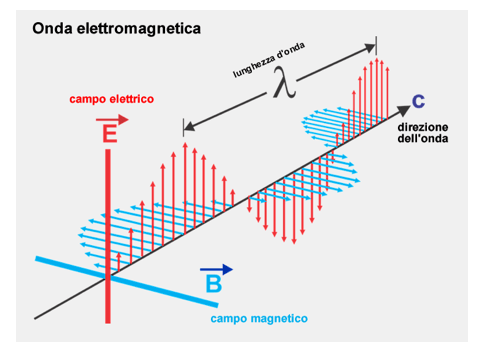
\includegraphics[width=5cm]{onda-elettromagnetica.png}
        %\label{fig:my_label1}
        \caption*{Polarizzazione lineare.}
     \end{figure}
\end{minipage}
\begin{minipage}{0.5\textwidth}
    \vspace{0.3cm}\begin{figure}[H]
        \centering
        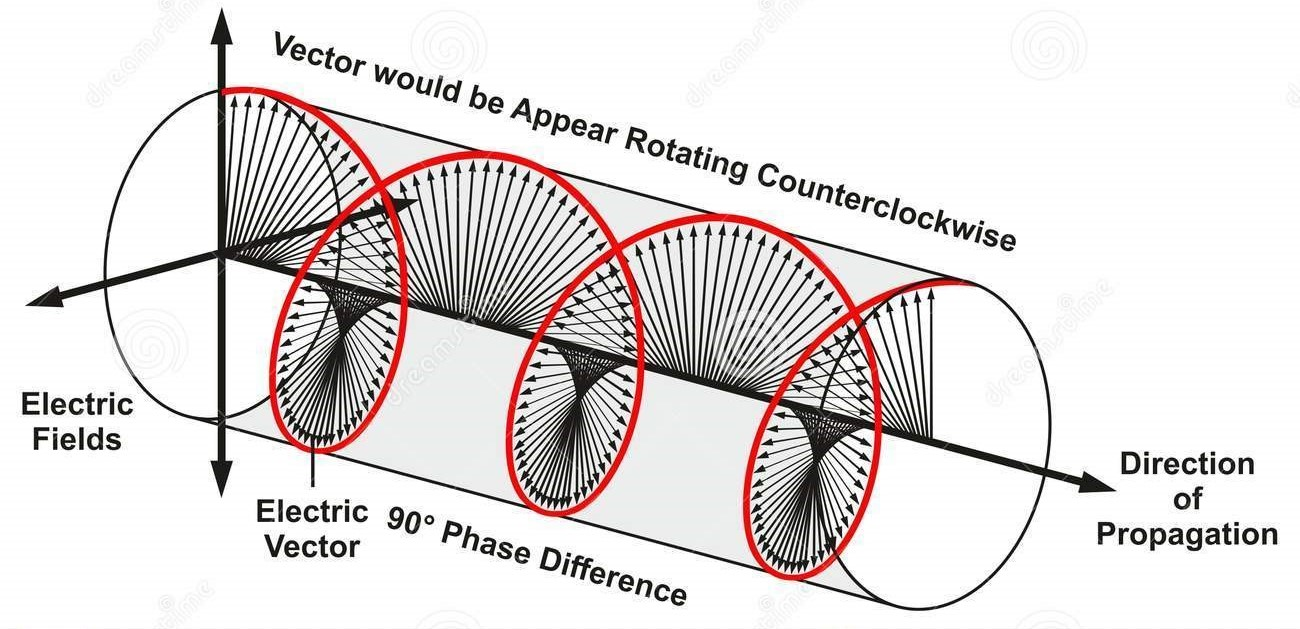
\includegraphics[width=7cm]{pol circ.jpg}
        %\label{fig:my_label2}
        \caption*{Polarizzazione circolare.}
    \end{figure}
\end{minipage}

\vspace{0.3cm}Il sensore interpreta queste variazioni e le converte in segnali attraverso opportuni processi.

Per frequenze nell'ordine di grandezza della luce visibile non esistono ancora sensori in grado di rilevare con precisione la fase della radiazione luminosa perché troppo piccola (varia nell' o.d.g. di $10^{15}$ volte al secondo); è per questo motivo che nello studio di queste onde consideriamo solo i valori medi di tali grandezze, operando un integrale sulla parte temporale dell'equazione dell'onda ed osservando così le sole variazioni spaziali del campo elettrico.

\vspace{0.2cm}La radiazione contiene informazioni sulla sorgente che l'ha prodotta, per cui in astrofisica si cerca di estrarre dalla radiazione la "firma" che la sorgente ha lasciato sulla radiazione. Essa prende un nome a seconda della lunghezza d'onda da essa posseduta. Nell'immagine seguente, sono riportate le tipologie di radiazioni principali e i relativi intervalli di lunghezza d'onda (e frequenza) entro cui ricadono:

\begin{figure}[h!!]
    \centering
    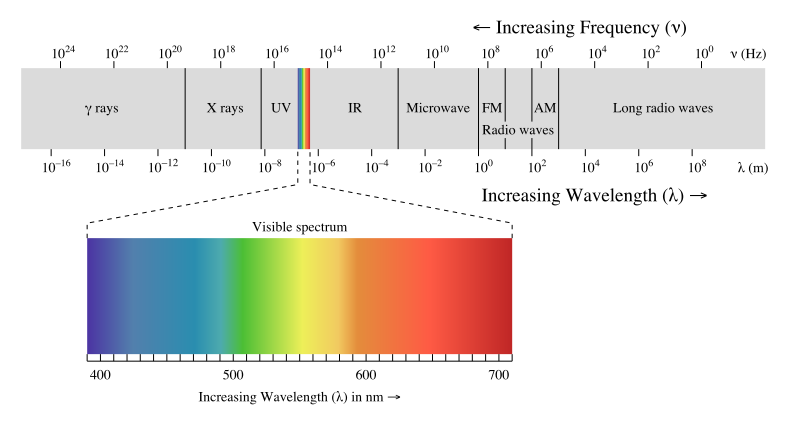
\includegraphics[width=10cm]{spettro em.png}
    %\label{fig:my_label3}
\end{figure}

Di tutto ciò che potrebbe essere potenzialmente emesso da una sorgente sotto forma di onda e.m., l'occhio umano vede solo quella parte che va dai 400 nm ai 700 nm, che prende il nome di \textit{luce visibile}.

Vorremmo ora quantificare l'energia trasportata da ognuna delle singole lunghezze d'onda, ovvero l'energia associata ad una specifica radiazione. Tale analisi quantitativa fu condotta per la prima volta alla fine del 1700 da Sir William Herschel, astronomo che misurò il primo spettro solare della storia. Scomponendo, infatti, la luce solare in diversi colori attraverso l'uso di un prisma, Sir Herschel pose un termometro su ogni colore e ne misurò la temperatura (esprimente una forma di energia) in funzione della lunghezza d'onda del colore. Inoltre, posizionando un termometro \textit{vicino} al colore rosso (ma non sulla parte di piano illuminata da esso), si accorse che anche questo si riscaldava e, quindi, intuì l'esistenza della radiazione "infrarossa" (intendendo un'onda con frequenza superiore a quella del rosso, non visibile all'occhio umano).

\begin{minipage}{0.395\textwidth}
    \begin{figure}[H]
        \centering
        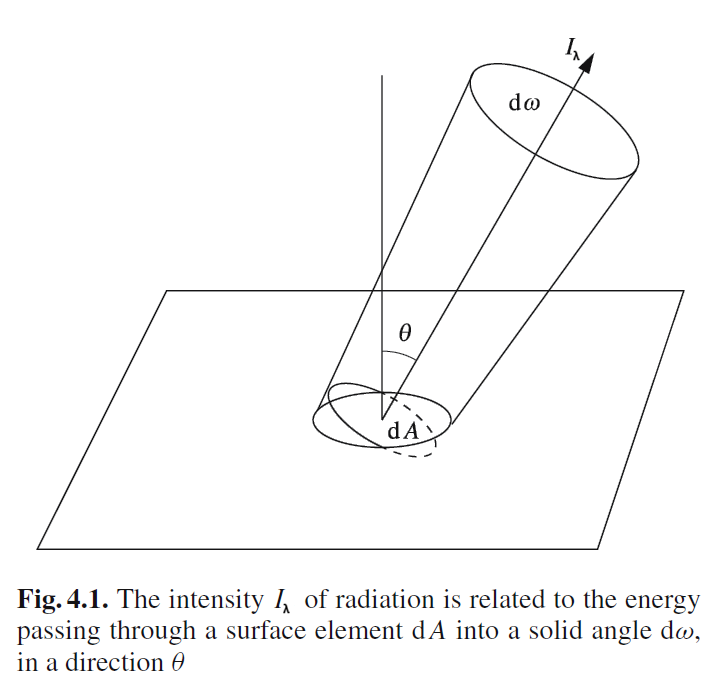
\includegraphics[width=5cm]{immagini/intensita_specifica_area.png}
    \end{figure}
\end{minipage}
\begin{minipage}{0.6\textwidth}
    In astrofisica, per quantificare l'energia usiamo una grandezza detta \textbf{intensità specifica} per unità di lunghezza d'onda, ovvero la quantità di energia che attraversa una superficie infinitesima $dA$ data quella particolare $\lambda$:

    \begin{equation}
        I_{\lambda}(\theta,\phi)d\lambda
        = \frac{dE_{\lambda}d\lambda}{dtdA\cos{\theta}d\omega}
    \end{equation}
\end{minipage}

\vspace{0.2cm}La precedente definizione d'intensità specifica normalizza l'energia nell'unità di tempo $dt$ e tiene anche conto dell'orientamento della superficie rispetto alla direzione di propagazione dell'onda incidente: quindi, non si normalizza tanto per l'area infinitesima $dA$, quanto per l'area proiettata lungo la direzione di propagazione dell'onda $dA\cos{\theta}$. Infine, è necessario anche tenere conto dell'estensione della superficie soggetta alla radiazione e, quindi, dell'angolo solido $d\omega$ con cui la sorgente puntiforme vede la superficie.

La definizione di intensità specifica può essere espressa anche in unità di frequenza:

\begin{equation}
    I_{\nu}(\theta,\phi)d\nu = \frac{dE_{\nu}d\nu}{dtdA\cos{\theta}d\omega}
\end{equation}

Una importante proprietà dell'intensità specifica afferma che questa grandezza \textit{non dipende dalla distanza}. Consideriamo infatti due superfici $dA$ e $dA'$ molto distanti tra loro, e gli angoli $\theta$ e $\theta'$ con cui una superficie vede l'altra:

\begin{figure}[H]
   \centering
   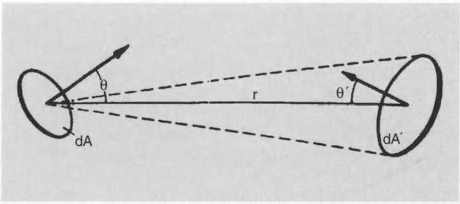
\includegraphics[width=8cm]{immagini/intensita_specifica.png}
\end{figure}

Essendo $dA\cos{\theta}$ e $dA'\cos{\theta'}$ le proiezioni di due superfici infinitesime sulla medesima direzione (quella individuata dalla congiungente), queste due quantità possono essere considerate uguali e, ricordando la definizione di angolo solido $d\omega$, si giunge alla conclusione che \textit{l'intensità specifica della radiazione incidente su entrambe $dA$ e $dA'$ è la stessa}, cioè è indipendente dalle distanze e dipende solo dagli angoli con cui le due superfici si guardano.

\vspace{0.2cm}Nota: ciò è vero solo se non sono presenti altre sorgenti o corpi assorbenti nello spazio compreso tra $dA$ e $dA'$.

\vspace{0.2cm}Questo significa che, ad esempio, l'intensità specifica della radiazione solare che emerge da una porzione di superficie del sole è la stessa di quella che arriva ad un telescopio sulla Terra che guarda quella stessa porzione di superficie. Inoltre spesso in astrofisica non si ha la percezione delle distanze: non riusciamo a capire se un oggetto è più o meno lontano, ecco perché è utile che non dipenda dalla distanza.

\vspace{0.2cm}Quello che gli astronomi misurano nella pratica con i loro strumenti è la \textbf{luminosità} del corpo celeste, definita come la quantità di energia della radiazione incidente nell'unità di tempo:

\begin{equation}
    L=\frac{dE}{dt}
\end{equation}

Definiamo poi il \textbf{flusso} di una sorgente a distanza $d$ come

\begin{equation}
    F=\frac{L}{4\pi d^2}
\end{equation}

che ci permette di legare la luminosità che misuriamo con i telescopi alla sorgente emettitrice.

Da tale relazione deduciamo che, approssimando le sorgenti ad oggetti puntiformi, il flusso dell'onda diminuisce nello spazio come fa la superficie di una sfera di raggio pari alla distanza $d$ dalla sorgente.

\begin{figure}[H]
    \centering
    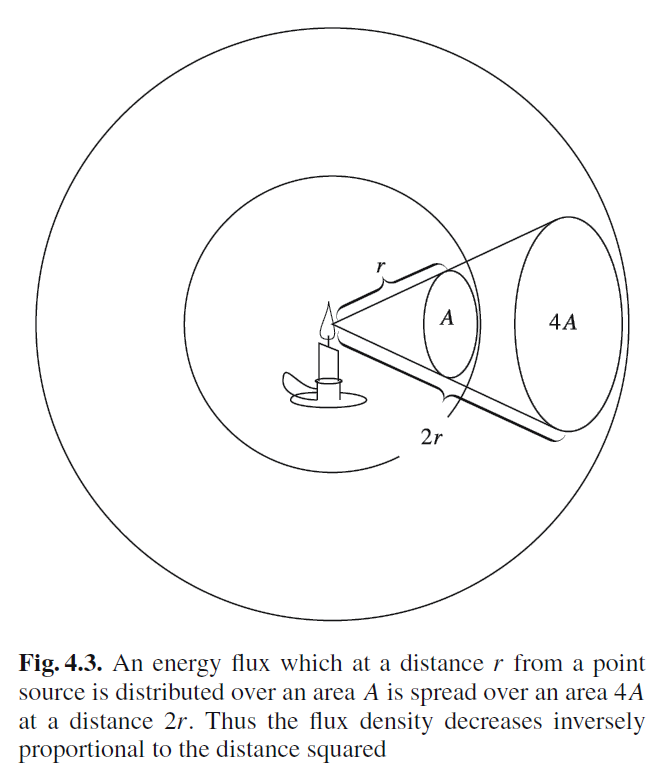
\includegraphics[width=6cm]{immagini/flusso_radiazione.png}
\end{figure}

Se le sorgenti piuttosto che essere puntiformi avessero delle dimensioni non trascurabili, la luminosità e il flusso diventerebbero funzioni delle coordinate del punto della sorgente preso in considerazione. Definiamo, infine, la \textbf{brillanza superficiale} di una sorgente estesa come la \textit{somma} di tutti i possibili contributi al flusso dati dai vari punti della superficie della sorgente.